
% Template for Elsevier CRC journal article
% version 1.2 dated 09 May 2011

% This file (c) 2009-2011 Elsevier Ltd.  Modifications may be freely made,
% provided the edited file is saved under a different name

% This file contains modifications for Procedia Computer Science
% but may easily be adapted to other journals

% Changes since version 1.1
% - added "procedia" option compliant with ecrc.sty version 1.2a
%   (makes the layout approximately the same as the Word CRC template)
% - added example for generating copyright line in abstract

%-----------------------------------------------------------------------------------

%% This template uses the elsarticle.cls document class and the extension package ecrc.sty
%% For full documentation on usage of elsarticle.cls, consult the documentation "elsdoc.pdf"
%% Further resources available at http://www.elsevier.com/latex

%-----------------------------------------------------------------------------------

%%%%%%%%%%%%%%%%%%%%%%%%%%%%%%%%%%%%%%%%%%%%%%%%%%%%%%%%%%%%%%
%%%%%%%%%%%%%%%%%%%%%%%%%%%%%%%%%%%%%%%%%%%%%%%%%%%%%%%%%%%%%%
%%                                                          %%
%% Important note on usage                                  %%
%% -----------------------                                  %%
%% This file should normally be compiled with PDFLaTeX      %%
%% Using standard LaTeX should work but may produce clashes %%
%%                                                          %%
%%%%%%%%%%%%%%%%%%%%%%%%%%%%%%%%%%%%%%%%%%%%%%%%%%%%%%%%%%%%%%
%%%%%%%%%%%%%%%%%%%%%%%%%%%%%%%%%%%%%%%%%%%%%%%%%%%%%%%%%%%%%%

%% The '3p' and 'times' class options of elsarticle are used for Elsevier CRC
%% Add the 'procedia' option to approximate to the Word template
%\documentclass[3p,times,procedia]{elsarticle}
\documentclass[3p,times]{elsarticle}
\usepackage[spanish]{babel}
%% The `ecrc' package must be called to make the CRC functionality available
\usepackage{ecrc}
\usepackage{hyperref}
%\usepackage[numbers,sort&compress]{natbib}

\usepackage{algorithm} 
\usepackage{algpseudocode} 
\usepackage{listings}
\usepackage[flushleft]{threeparttable}
\usepackage{booktabs}

\newenvironment{abstracts}
 {\global\setbox\absbox=\vbox\bgroup
    \hsize=\textwidth
    \linespread{1}\selectfont}
 {\vspace{-\bigskipamount}\egroup}
\renewenvironment{abstract}[1][]
 {\if\relax\detokenize{#1}\relax\else\selectlanguage{#1}\fi
  \noindent\textbf{\abstractname}\par\medskip\noindent\ignorespaces}
 {\par\bigskip}
\let\today\relax
\makeatletter
\def\ps@pprintTitle{%
    \let\@oddhead\@empty
    \let\@evenhead\@empty
    \def\@oddfoot{\footnotesize\itshape
         {} \hfill\today}%
    \let\@evenfoot\@oddfoot
    }
\makeatother
\makeatletter
\renewcommand*{\ALG@name}{Algoritmo}

%% The ecrc package defines commands needed for running heads and logos.
%% For running heads, you can set the journal name, the volume, the starting page and the authors

%% set the volume if you know. Otherwise `00'
%\volume{00}

%% set the starting page if not 1
\firstpage{1}

%% Give the name of the journal
\journalname{Procedia Computer Science}

%% Give the author list to appear in the running head
%% Example \runauth{C.V. Radhakrishnan et al.}
%\runauth{}

%% The choice of journal logo is determined by the \jid and \jnltitlelogo commands.
%% A user-supplied logo with the name <\jid>logo.pdf will be inserted if present.
%% e.g. if \jid{yspmi} the system will look for a file yspmilogo.pdf
%% Otherwise the content of \jnltitlelogo will be set between horizontal lines as a default logo

%% Give the abbreviation of the Journal.  Contact the journal editorial office if in any doubt
\jid{procs}

%% Give a short journal name for the dummy logo (if needed)
%\jnltitlelogo{Procedia Computer Science}

%% Provide the copyright line to appear in the abstract
%% Usage:
%   \CopyrightLine[<text-before-year>]{<year>}{<restt-of-the-copyright-text>}
%   \CopyrightLine[Crown copyright]{2011}{Published by Elsevier Ltd.}
%   \CopyrightLine{2011}{Elsevier Ltd. All rights reserved}
\CopyrightLine{2011}{Published by Elsevier Ltd.}

%% Hereafter the template follows `elsarticle'.
%% For more details see the existing template files elsarticle-template-harv.tex and elsarticle-template-num.tex.

%% Elsevier CRC generally uses a numbered reference style
%% For this, the conventions of elsarticle-template-num.tex should be followed (included below)
%% If using BibTeX, use the style file elsarticle-num.bst

%% End of ecrc-specific commands
%%%%%%%%%%%%%%%%%%%%%%%%%%%%%%%%%%%%%%%%%%%%%%%%%%%%%%%%%%%%%%%%%%%%%%%%%%

%% The amssymb package provides various useful mathematical symbols
\usepackage{amssymb}
%% The amsthm package provides extended theorem environments
%% \usepackage{amsthm}

%% The lineno packages adds line numbers. Start line numbering with
%% \begin{linenumbers}, end it with \end{linenumbers}. Or switch it on
%% for the whole article with \linenumbers after \end{frontmatter}.
%% \usepackage{lineno}

%% natbib.sty is loaded by default. However, natbib options can be
%% provided with \biboptions{...} command. Following options are
%% valid:

%%   round  -  round parentheses are used (default)
%%   square -  square brackets are used   [option]
%%   curly  -  curly braces are used      {option}
%%   angle  -  angle brackets are used    <option>
%%   semicolon  -  multiple citations separated by semi-colon
%%   colon  - same as semicolon, an earlier confusion
%%   comma  -  separated by comma
%%   numbers-  selects numerical citations
%%   super  -  numerical citations as superscripts
%%   sort   -  sorts multiple citations according to order in ref. list
%%   sort&compress   -  like sort, but also compresses numerical citations
%%   compress - compresses without sorting
%%
%% \biboptions{comma,round}

% \biboptions{}

% if you have landscape tables
\usepackage[figuresright]{rotating}

% put your own definitions here:
%   \newcommand{\cZ}{\cal{Z}}
%   \newtheorem{def}{Definition}[section]
%   ...

% add words to TeX's hyphenation exception list
%\hyphenation{author another created financial paper re-commend-ed Post-Script}

% declarations for front matter

\begin{document}

\begin{frontmatter}

%% Title, authors and addresses

%% use the tnoteref command within \title for footnotes;
%% use the tnotetext command for the associated footnote;
%% use the fnref command within \author or \address for footnotes;
%% use the fntext command for the associated footnote;
%% use the corref command within \author for corresponding author footnotes;
%% use the cortext command for the associated footnote;
%% use the ead command for the email address,
%% and the form \ead[url] for the home page:
%%
%% \title{Title\tnoteref{label1}}
%% \tnotetext[label1]{}
%% \author{Name\corref{cor1}\fnref{label2}}
%% \ead{email address}
%% \ead[url]{home page}
%% \fntext[label2]{}
%% \cortext[cor1]{}
%% \address{Address\fnref{label3}}
%% \fntext[label3]{}

%\dochead{}
%% Use \dochead if there is an article header, e.g. \dochead{Short communication}
%% \dochead can also be used to include a conference title, if directed by the editors
%% e.g. \dochead{17th International Conference on Dynamical Processes in Excited States of Solids}

\title{Relación entre el número de ingresos hospitalarios y los niveles de contaminación}

%% use optional labels to link authors explicitly to addresses:
%% \author[label1,label2]{<author name>}
%% \address[label1]{<address>}
%% \address[label2]{<address>}

\author{Selene Berenice Prado Prado}

\address{San Nicolás de los Garza, Nuevo León, México}

%\begin{abstract}
%% Text of abstract
%\end{abstract}
\begin{abstracts}
\begin{abstract}[spanish]

El objetivo de la investigación es generar modelos que permitan visualizar relaciones entre contaminantes atmosféricos y salud pública. Los modelos generados se utilizan en conjunto con datos obtenidos de la Secretaría de Salud del Gobierno de México y registros de los niveles de los contaminantes presentes en el área metropolitana de Monterrey.

El tener un modelo que permita visualizar relaciones entre contaminantes atmosféricos y salud pública que sea utilizado con datos confiables y verídicos pueden ayudar a entender el impacto que tiene el aumento del nivel de contaminantes atmosféricos.

Este trabajo comprende el procedimiento  realizado para generar un inventario forestal de dos áreas forestales: el cilantrillo y la trinidad. En dichas zonas es clasificada cada una de las especies detectadas en las muestras recolectadas de su respectiva zona forestal, generando así, el inventario forestal por medio del procesamiento de imágenes.
\end{abstract}

\textit{Palabras clave: } Aprendizaje máquina, Ciencia de datos, Contaminante del aire, Regresión lineal, Salud, Semana epidemiológica, Serie de tiempo.
\vspace*{0.5cm}
\end{abstracts}

%\begin{keyword}
%% keywords here, in the form: keyword \sep keyword

%% PACS codes here, in the form: \PACS code \sep code

%% MSC codes here, in the form: \MSC code \sep code
%% or \MSC[2008] code \sep code (2000 is the default)

%\end{keyword}

\end{frontmatter}

%%
%% Start line numbering here if you want
%%
% \linenumbers

%% main text
\section{Introducción}
%\label{}
El \emph{aprendizaje máquina}\footnote{Traducido como \emph{machine learning} en inglés, tiene como objetivo desarrollar técnicas que les permitan a las computadoras aprender.} es un área dentro de la \emph{ciencia de datos}\footnote{Traducido como \emph{data science} en inglés, involucra métodos para extraer conocimiento de datos, eso con la finalidad de que haya un mejor entendimiento de los datos.} que puede ayudar a crear dichos modelos para tener una más eficiente visualización cuando se trabaja con una gran cantidad de datos, que es lo que se requiere para el presente trabajo. El área de la ciencia de datos es muy útil ya que permite trabajar con grandes cantidades de datos aminorando la cantidad de tiempo empleado en la creación de gráficos que permitan visualizar los datos. El crear modelos para la visualización de datos ayuda a observar con mayor claridad los datos para encontrar relaciones entre ellos.

La tarea en el presente proyecto es utilizar modelos para visualizar las relaciones entre los contaminantes del aire y salud pública. Para la realización de los experimentos se tienen datos de ingresos hospitalarios provenientes de la base de datos de la Secretaría de Salud del Gobierno de México \cite{f1}. También se tienen registros de los niveles de algunos contaminantes del aire presentes en el área metropolitana de Monterrey, capturados por las estaciones de monitoreo pertenecientes al Sistema Integral de Monitoreo Ambiental (SIMA) \cite{f2} mostradas en la figura \ref{estaciones}.

\begin{figure}[h!]
\setcounter{figure}{0} % por culpa de sciposter
%\captionsetup{type=figure} % por culpa de sciposter
\begin{center}
   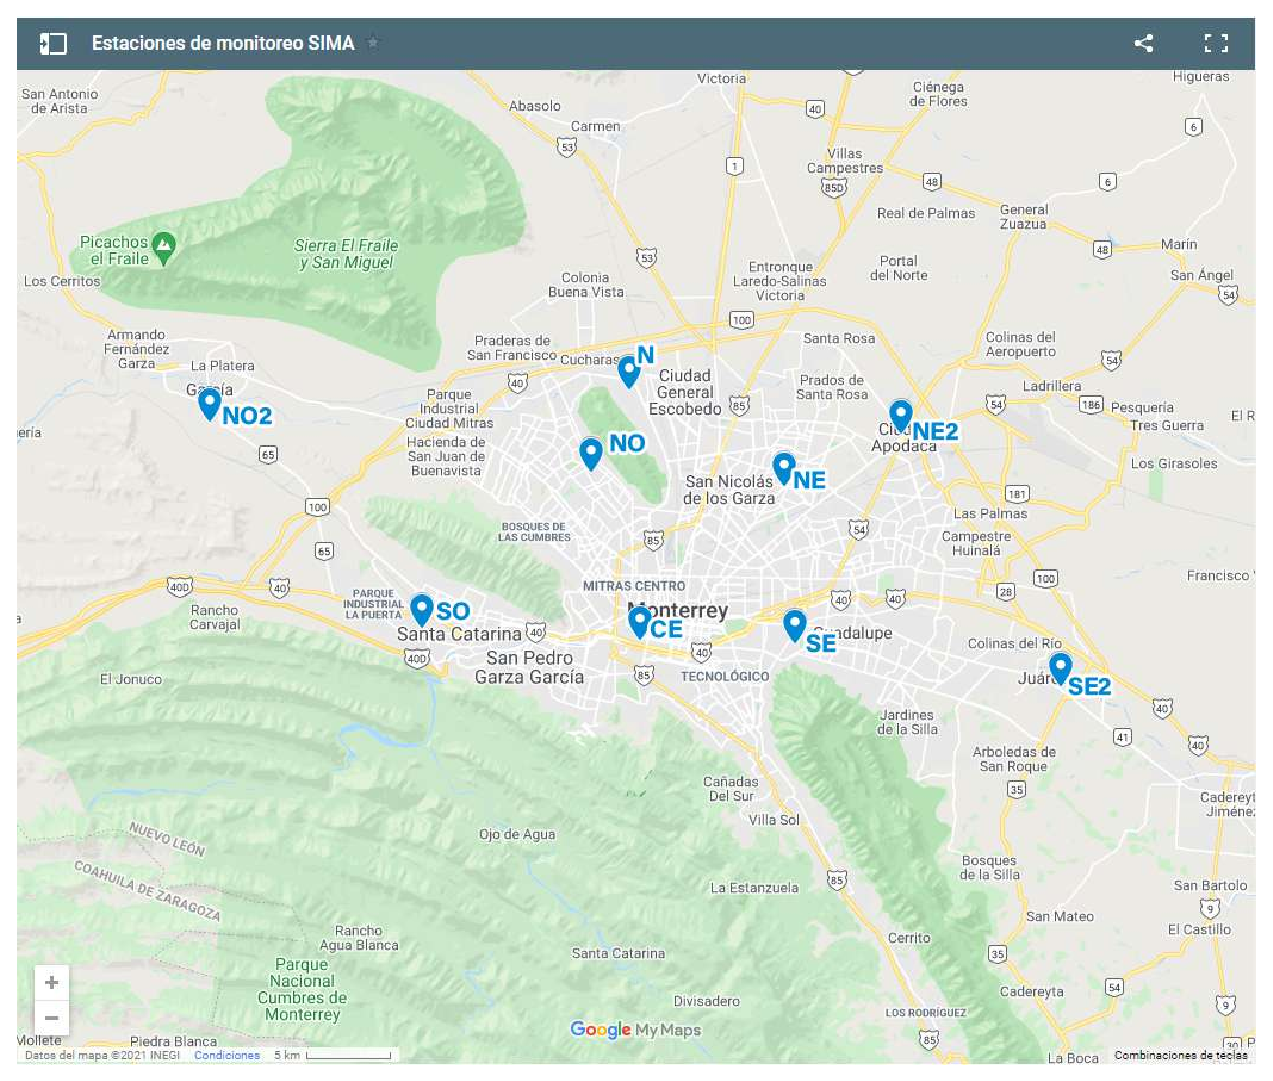
\includegraphics[trim=50 50 50 50,clip,width=0.5\textwidth]{mapa_estaciones.eps}
   \end{center}
    \caption{Localización de las estaciones de monitoreo de la calidad del aire.}
    \label{estaciones}
\end{figure}

\subsection{Motivación}
Existen investigaciones que ya han estudiado las relaciones entre contaminantes del aire y salud pública, sin embargo, con el presente trabajo se busca aportar a la creación de nuevas herramientas que permitan observar y estudiar dichas relaciones con el fin de ayudar a tomar medidas adecuadas que permitan aminorar los efectos negativos de los contaminantes del aire en la salud.

\subsection{Hipótesis}
Los modelos de regresión permiten obtener gráficos donde se pueden observar las relaciones entre el número de ingresos hospitalarios y los niveles de contaminantes del aire.

\subsection{Objetivos}
El objetivo de generar, implementar y evaluar modelos que muestran las relaciones existentes entre contaminantes del aire y salud pública tiene la finalidad de apoyar a la implementación de estrategias que aminoran los efectos negativos de los contaminantes del aire en la salud de las personas. Con los modelos generados se puede tener una herramienta que permite identificar gráficamente las relaciones con solo proporcionarle el conjunto de datos.


\section{Antecedentes}

Existen factores ambientales que afectan la salud de una comunidad como: el abastecimiento de agua potable y el saneamiento, la vivienda y el hábitat, la alimentación, la contaminación ambiental, el empleo de productos químicos y los riesgos ocupacionales \citep{r2}. 

Contaminación del aire es un término usado para describir la presencia de uno o más contaminantes en la atmósfera, cuyas cantidades y características pueden resultar perjudiciales o interferir con la salud, el bienestar u otros procesos ambientales naturales \citep{r3}.

\subsection{Monitoreo de calidad del aire}
Existen diversos estudios que muestran la existencia de potenciales efectos a la salud cuando en el aire están presentes contaminantes en forma de partículas, gases o agentes biológicos.
%En los últimos años ha habido un desarrollo considerable de la tecnología para el control de la calidad del aire, esto como resultado de una mayor conciencia, tanto de parte de los gobiernos como de los ciudadanos, sobre la importancia de mantener el aire lo más apto posible para la vida humana.

\citet{r4} mencionan que desde inicios de 1950 se observa una preocupación por los contaminantes del aire  en los países de América Latina y el Caribe. Las universidades y dependencias de los ministerios de salud fueron los organismos que realizaron las primeras mediciones de contaminación en el aire.

En 1965, el Consejo Directivo de la Organización Panamericana de la Salud (OPS) recomendó el establecer programas de investigación de la contaminación del agua y del aire, con el objetivo de colaborar en el desarrollo de políticas adecuadas de control \citep{r5}.

Mediante el Centro Panamericano de Ingeniería Sanitaria y Ciencias del Ambiente (CEPIS), la OPS acordó establecer una red de estaciones de muestreo de la contaminación del aire.
En junio de 1967 la Red Panamericana de Muestreo Normalizado de la Contaminación del Aire (REDPANAIRE) inició sus operaciones recolectando muestras diarias de partículas totales en suspensión (PTS) y de SO$_2$. La REDPANAIRE comenzó con ocho estaciones y a fines de 1973 tenía un total de 88 estaciones distribuidas en 26 ciudades de 14 países \citep{r5}.

Para diciembre de 1973 se habían recolectado más de 350,000 datos sobre la calidad del aire, en los que se observa que algunas ciudades mostraban una tendencia al incremento de los niveles de contaminación \citep{r5}.

En 1980 la REDPANAIRE desapareció y pasó a formar parte del Programa Global de Monitoreo de la Calidad del Aire, iniciado en 1976 por la OMS y el Programa de las Naciones Unidas para el Medio Ambiente (PNUMA), como parte de un sistema global de monitoreo ambiental llamado GEMS por sus siglas en inglés \emph{Global Environmental Monitoring System}.

En la década de 1990, la OMS instituyó, con carácter global, el Sistema de Información para el Control de la Calidad del Aire llamado AMIS por sus siglas en inglés \emph{Air Management Information System}. Entre las actividades más destacadas de AMIS se incluye el coordinar las bases de datos sobre temas relacionados con la calidad del aire.

En Nuevo León, México, las operaciones de la Red Automática de Monitoreo Atmosférico iniciaron en 1993. Dicha red en sus inicios contaba con cinco estaciones fijas de monitoreo continuo de monóxido de carbono (CO), dióxido de azufre (SO$_2$), óxidos de nitrógeno (NO$_x$), ozono (O$_3$) y partículas de tamaño menor a 10 micrómetros (PM10) \citep{r4}. Como se muestra en la figura \ref{estaciones}, actualmente se cuenta con nueve estaciones fijas.

\subsection{Series de tiempo}
\citet{r4} mencionan que las relaciones entre niveles de concentraciones de contaminantes del aire y los efectos sobre la salud generalmente son obtenidas de estudios epidemiológicos de series de tiempo. Uno de los diseños epidemiológicos más utilizados son los estudios de series temporales. Con esos diseños se analizan las variaciones en el tiempo de la exposición al contaminante y el indicador de salud estudiado en una población \citep{r1}.

Las series de tiempo se pueden definir como un conjunto de observaciones {{ot}} tomadas en un tiempo $t$ determinado. Los estudios de series de tiempo relacionan estadísticamente los cambios temporales en la repercusión de cambios en la concentración de un contaminante en la población \citep{r8}.

Para mostrar datos en una serie de tiempo, especialmente en el área médica, estos suelen agruparse en \emph{semanas epidemiológicas}\footnote{Una semana epidemiológica es un estándar de medición temporal que se utiliza para comparar datos en ventanas de tiempo definidas. La primera semana epidemiológica del año termina el primer sábado de enero de cada año \citep{r7}.}. 

\subsection{Clasificación de enfermedades}
Existe un instrumento estadístico y sanitario para identificar enfermedades llamado Clasificación Internacional de Enfermedades (CIE), cuya finalidad es entender las causas de morbilidad y mortalidad de la población y así mejorar la calidad de vida de la misma. Es en base a un criterio epidemiológico y sanitario establecido por Farr a finales del siglo XIX que esta clasificación agrupa enfermedades en epidémicas, generales, locales ordenadas por origen geográfico, trastornos del desarrollo y lesiones \citep{r9}. Para lograr distinguirlas se emplea un código alfanumérico que consiste de una letra en la primera posición, seguida de dos dígitos, un punto decimal y un último dígito. El rango de valores va de A00.0 a Z99.9.

\subsection{Regresión lineal}
La tendencia $w_0$ de una serie de tiempo puede ser obtenida a partir de una regresión lineal de la misma \citep{r10}. Una regresión lineal es una metodología inferencial supervisada que busca predecir valores $y$ dado un vector de variables de entrada $t$ por medio del ajuste de coeficientes $w$ de la función lineal 
\begin{equation}
    \hat{y}(t,w) = w_0 + w_1x_1 + ... + w_tx_t.
    \label{eq1}
\end{equation}

\subsection{Regresión lineal múltiple}
Un modelo de regresión múltiple es un modelo complemento de la regresión lineal simple, el cual tiene dos o más variables independientes $k$ que pueden influir en una variable dependiente $y$. \citet{r11} expresan la regresión múltiple mediante la siguiente ecuación:
\begin{equation}
    y = \beta_0 + \beta_1x_1 + ... + \beta_kx_k + \varepsilon.
    \label{eq2}
\end{equation}



\section{Estado del arte}

Se recopila literatura relacionada desde el año 2017 hasta el año 2021. En esta sección los trabajos se mencionan en orden cronológico tomando en cuenta su año de publicación.

\citet{r12} estudian la relación entre los niveles de contaminantes ambientales y la presencia de casos de enfermedades respiratorias en las consultas pediátricas. La variable dependiente analizada es la demanda en las consultas pediátricas por bronquiolitis, episodios de broncoespasmo y procesos respiratorios de vías altas. Como variables independientes se tienen los valores de contaminación ambiental. Se calculan coeficientes de correlación y regresión lineal múltiple.

\citet{r13} abordan la necesidad de monitoreo, control y predicción de la pendiente de los niveles de contaminantes del aire. Para abordar el problema de investigación utilizan modelos ARIMA. 

\citet{r14} estudian la asociación entre la exposición a largo plazo a la contaminación del aire y la metilación del ADN. Para ello realizan un estudio utilizando modelos de regresión lineal robustos para analizar la asociación entre la exposición al NO$_2$ y a las partículas PM10 y PM2.5.

\citet{r15} en su estudio abordan los niveles de contaminación del aire y su asociación con la presencia de presión sanguínea elevada en niños y adolescentes. La exposición a partículas PM10 y PM2.5 son estimadas con un modelo espacio-temporal. Son utilizados modelos lineales de efectos mixtos y modelos de regresión logística para investigar la asociación entre la exposición a partículas PM y presión sanguínea e hipertensión. 

\citet{r16} estudian la relación entre los niveles de contaminación del aire y la obesidad y problemas cardiometabólicos. Para dicho estudio emplean modelos de regresión lineal.

\citet{r17} examinan las asociaciones entre la exposición temprana a la contaminación del aire y la incidencia de asma y rinitis alérgica desde el nacimiento hasta la adolescencia. Para su estudio utilizan modelos de regresión.

\citet{r18} estudian la asociación entre la exposición temprana a los contaminantes del aire y los egresos hospitalarios por asma. Para su estudio aplican modelos de regresión logística para el análisis de datos. 

\citet{r19} abordan el estudio de la relación entre los niveles de contaminación del aire y el número de admisiones hospitalarias. Para ello se construye un modelo basado en la distribución de Poisson.

\citet{r20} estudian la relación entre la mortalidad del coronavirus (COVID-19) y la contaminación del aire. Para dicho estudio emplean un modelo de regresión lineal para establecer la relación entre los parámetros de la contaminación del aire (concentraciones de PM10 o PM2.5) y la variable de respuesta (porcentaje de mortalidad por unidad de casos reportados).

\subsection{Comparación de trabajos}
La mayoría de los trabajos encontrados emplean modelos de regresión lineal o modelos de predicción. Además, en todos los trabajos encontrados el problema tratado presenta una alta relación con el problema abordado en el presente trabajo de tesis. El análisis comparativo de los trabajos relacionados se hace en base de los siguientes puntos:

\begin{description}
\item[Modelos de regresión lineal:]{Son aquellos que ayudan a estudiar la relación entre una variable dependiente y una o más variables independientes.}
\end{description}

\begin{description}
\item[Modelos de predicción:]{Son aquellos que ayudan a hacer predicciones de una variable.}
\end{description}

\begin{description}
\item[Evaluación de modelos:]{Se refiere a la utilización de técnicas para evaluar la eficacia de los modelos generados.}
\end{description}

\begin{description}
\item[Estudio de contaminantes del aire:]{Se refiere a que el tema de estudio incluya uno o más contaminantes del aire.}
\end{description}

\begin{description}
\item[Estudio de problemas de salud:]{Se refiere a que el tema de estudio incluya uno o más problemas de salud.}
\end{description}

En el cuadro \ref{tab:Comparación de trabajos frente al desarrollado} se desglosan las características presentes que se pueden encontrar en las investigaciones citadas y su relación con la investigación con la que se está trabajando actualmente.

\begin{table}[hbt!]
\centering
\caption[Comparación de trabajos]{Comparación de trabajos frente al desarrollado, donde $\checkmark$ indica que cumple con esta característica y  $\times$ no cumple con esta característica.}
\vspace{0.5cm}
%\begin{adjustbox}{width=0.5\textwidth}
\begin{tabular}{|l|c|c|c|c|c|}
\hline
Trabajo & \rotatebox[origin=c]{90}{ Modelos de regresión lineal } & \rotatebox[origin=c]{90}{ Modelos de predicción } & \rotatebox[origin=c]{90}{ Evaluación de modelos } & \rotatebox[origin=c]{90}{ Estudio de contaminantes del aire } & \rotatebox[origin=c]{90}{ Estudio de problemas de salud }\\
	\hline
    \citet{r12} & \checkmark & $\times$ & $\times$ & \checkmark & \checkmark\\
    \hline
    \citet{r13} &  $\times$ & \checkmark & \checkmark & \checkmark & $\times$\\
    \hline
    \citet{r14} & \checkmark & \checkmark & $\times$ & \checkmark & \checkmark\\
    \hline
    \citet{r15} & \checkmark & \checkmark & $\times$ & \checkmark & \checkmark\\
	\hline    
    \citet{r16}& \checkmark & $\times$ & $\times$ & \checkmark & \checkmark\\
	\hline    
    \citet{r17} & $\times$ & \checkmark & \checkmark & \checkmark & \checkmark\\
	\hline    
    \citet{r18} & $\times$  & $\times$ & $\times$ & \checkmark & \checkmark\\
	\hline    
    \citet{r19} & \checkmark & \checkmark & $\times$ & \checkmark & \checkmark\\
	\hline    
    \citet{r20} &  \checkmark & \checkmark & $\times$ & \checkmark & \checkmark\\
	\hline    
    El presente trabajo & \checkmark & \checkmark & \checkmark & \checkmark & \checkmark\\
    \hline
\end{tabular}
%\end{adjustbox}
\label{tab:Comparación de trabajos frente al desarrollado}
\end{table}

Como se puede observar en el cuadro \ref{tab:Comparación de trabajos frente al desarrollado}, la mayoría de los trabajos encontrados abordan el estudio de los contaminantes del aire y salud con excepción de \citet{r13} que se enfocan en la predicción de niveles de contaminantes del aire, lo cual puede indicar que la relación entre los contaminantes del aire y salud es un tema de relevancia en la actualidad. 

Ya que la mayoría de los trabajos encontrados estudian la relación entre contaminantes del aire y salud, la mayoría de los trabajos emplean modelos de regresión lineal por que es una buena opción para el estudio de relaciones entre variables. Las excepciones, además de la ya anteriormente mencionada, son \citet{r17} y \citet{r18} quienes emplean otros tipos de modelos de regresión.

En el presente trabajo se elaboran modelos de predicción para el tratamiento de los datos empleados para los experimentos, ya que como mencionan \citet{r15}, una de las limitaciones en este tipo de estudios es los campos sin llenar en los registros de datos.

En el presente trabajo también se emplean técnicas para evaluar los modelos generados. Solo en tres de los trabajos encontrados se aborda la evaluación de los modelos empleados, y al ser incluida en el presente estudio, puede representar una distinción.

\section{Solución propuesta}

En esta sección se plantean las herramientas utilizadas y los pasos seguidos para la solución propuestas. Las herramientas utilizadas en la presente investigación se muestran en el cuadro \ref{tab:Herramientas utilizadas}.

\begin{table}[h!]
	{\centering
		\caption{Herramientas utilizadas.}
		\vspace{0.5cm}
		\begin{tabular}{|c|c|c|}
			\hline 
			Herramienta & Versión & URL\\
			\hline
			\texttt{Python} & 3.8.8 & \url{https://www.python.org/}\\
			\hline
			\texttt{Jupyter Notebook} & 6.3.0 & \url{https://jupyter.org/}\\
			\hline
			\texttt{Imageio} & 2.9.0 & \url{https://imageio.readthedocs.io/}\\
			\hline
			\texttt{Latextable} & 0.2.1 & \url{https://pypi.org/project/latextable/}\\
			\hline
			\texttt{Matplotlib} & 3.3.4 & \url{https://matplotlib.org/}\\
			\hline
			\texttt{NumPy} & 1.20.1 & \url{http://www.numpy.org/}\\
			\hline
			\texttt{Pandas} & 1.2.4 & \url{https://pandas.pydata.org/}\\
			\hline
			\texttt{Seaborn} & 0.11.1 & \url{https://seaborn.pydata.org/}\\
			\hline
			\texttt{Scikit-learn} & 0.24.1 & \url{https://scikit-learn.org/}\\
			\hline
			\texttt{SciPy} & 1.6.2 & \url{https://docs.scipy.org/}\\
			\hline
			\texttt{Statsmodels} & 0.12.2 & \url{https://www.statsmodels.org/}\\
			\hline
			\texttt{Texttable} & 1.6.4 & \url{https://pypi.org/project/texttable/}\\
			\hline
		\end{tabular}
		
	\label{tab:Herramientas utilizadas}
	}
\end{table}

\subsection{Recolección de datos}
La primera fase es la recolección de datos. El objetivo es tener un archivo que contenga datos de los niveles de uno o más contaminantes del aire en años recientes y también del mismo lugar contar con datos del número de egresos hospitalarios durante esos años.

\subsection{Selección y agrupación de datos}
Después de la recolección de datos se seleccionan cuáles van a ser utilizados para los experimentos. Para ello se utiliza \texttt{Python} con la librería \texttt{Pandas} que permite la manipulación de datos. 
Para la selección y agrupación de datos se sigue el procedimiento mostrado en el algoritmo \ref{alg:a1}.

\begin{algorithm}
\caption{Selección y agrupamiento de datos}\label{alg:a1}
\begin{algorithmic}[1]
\State $a \leftarrow $ años de los que se obtuvieron datos
\For {$i \in a$}
    \State $contaminantes \leftarrow $ nombre del archivo .csv que contiene los datos de los contaminantes en el año $i$
    \State Leer en $contaminantes$ las columnas fecha y contaminante 
    \State $egresos \leftarrow $ nombre del archivo .csv que contiene los datos de los contaminantes en el año $i$
    \State Leer en $contaminantes$ las columnas fecha, padecimiento y estado
    \State $estado \leftarrow $ estado del que se quieren obtener datos
    \State Seleccionar en $contaminantes$ los datos del $estado$
\EndFor
\end{algorithmic} 
\end{algorithm}

\subsection{Visualización de la evolución de las variables}
Al ya tener seleccionados los datos a utilizar se procede a elaborar gráficos en \texttt{Python} que muestran la evolución de las variables en el tiempo. Para ello se generan los tipos de gráficos discutidos a continuación.

\subsubsection{Series de tiempo}
Se realizan series de tiempo en \texttt{Python} con ayuda de la librería  \texttt{Matplotlib}, \texttt{Scikit-learn} y \texttt{Seaborn}, ya que son herramientas accesibles que ayudan a la generación de este tipo de gráficos.

\subsubsection{Gráficos de radar}
Los gráficos de radar o diagramas de telaraña son otra manera de visualizar un conjunto de datos. Sirven para comparar variables visualizando si existen valores o patrones de evolución en el tiempo similares entre ellas. Es por ello que en el presente trabajo se elaboran gráficos de radar con ayuda de \texttt{Python} y las librerías \texttt{NumPy} y \texttt{Matplotlib}. En la figura \ref{grafico_de_telaraña} se muestra un ejemplo de los gráficos de telaraña generados.

\subsection{Implementación de modelos}
Después de haber generado gráficos para la visualización de la evolución de las variables, se procede a generar modelos para el estudio de la relación entre las variables. Para ello se utiliza \texttt{Python} y la librería \texttt{Statsmodels}. Los tipos de modelos generados se discuten a continuación.

\subsubsection{Regresión lineal}
Primeramente se calcula el coeficiente de correlación de Pearson y se verifica que esté entre -1 y 1. Si un valor es cercano a 0, quiere decir que no hay dependencia lineal. Si no hay una dependencia lineal no existe sustento para el modelo de regresión lineal. El modelo de regresión lineal arroja un valor de $R^2$ que indica en qué grado la variable independiente explica la varianza de la variable dependiente. Además, se obtiene el valor $p$ que indica la relevancia del resultado y se obtiene la raíz de error cuadrático medio (RMSE) que indica cuántas unidades se alejan los valores predichos por el modelo de los valores reales, eso ayuda a determinar el error del modelo.

\subsubsection{Regresión lineal múltiple}
En los modelos de regresión lineal múltiple se tiene más de una variable independiente. Primero se calcula el coeficiente de correlación de Pearson y se verifica que hay una dependencia lineal para generar el modelo de regresión lineal múltiple. El modelo arroja un valor de $R^2$ que indica en qué grado las variables independientes explican la varianza de la variable dependiente. Además, se obtiene el valor $p$ que indica la relevancia del resultado y se obtiene la raíz de error cuadrático medio (RMSE) que indica cuántas unidades se alejan los valores predichos por el modelo de los valores reales, eso ayuda a determinar el error del modelo.

\begin{figure}[h!]
\setcounter{figure}{1} % por culpa de sciposter
%\captionsetup{type=figure} % por culpa de sciposter
\begin{center}
   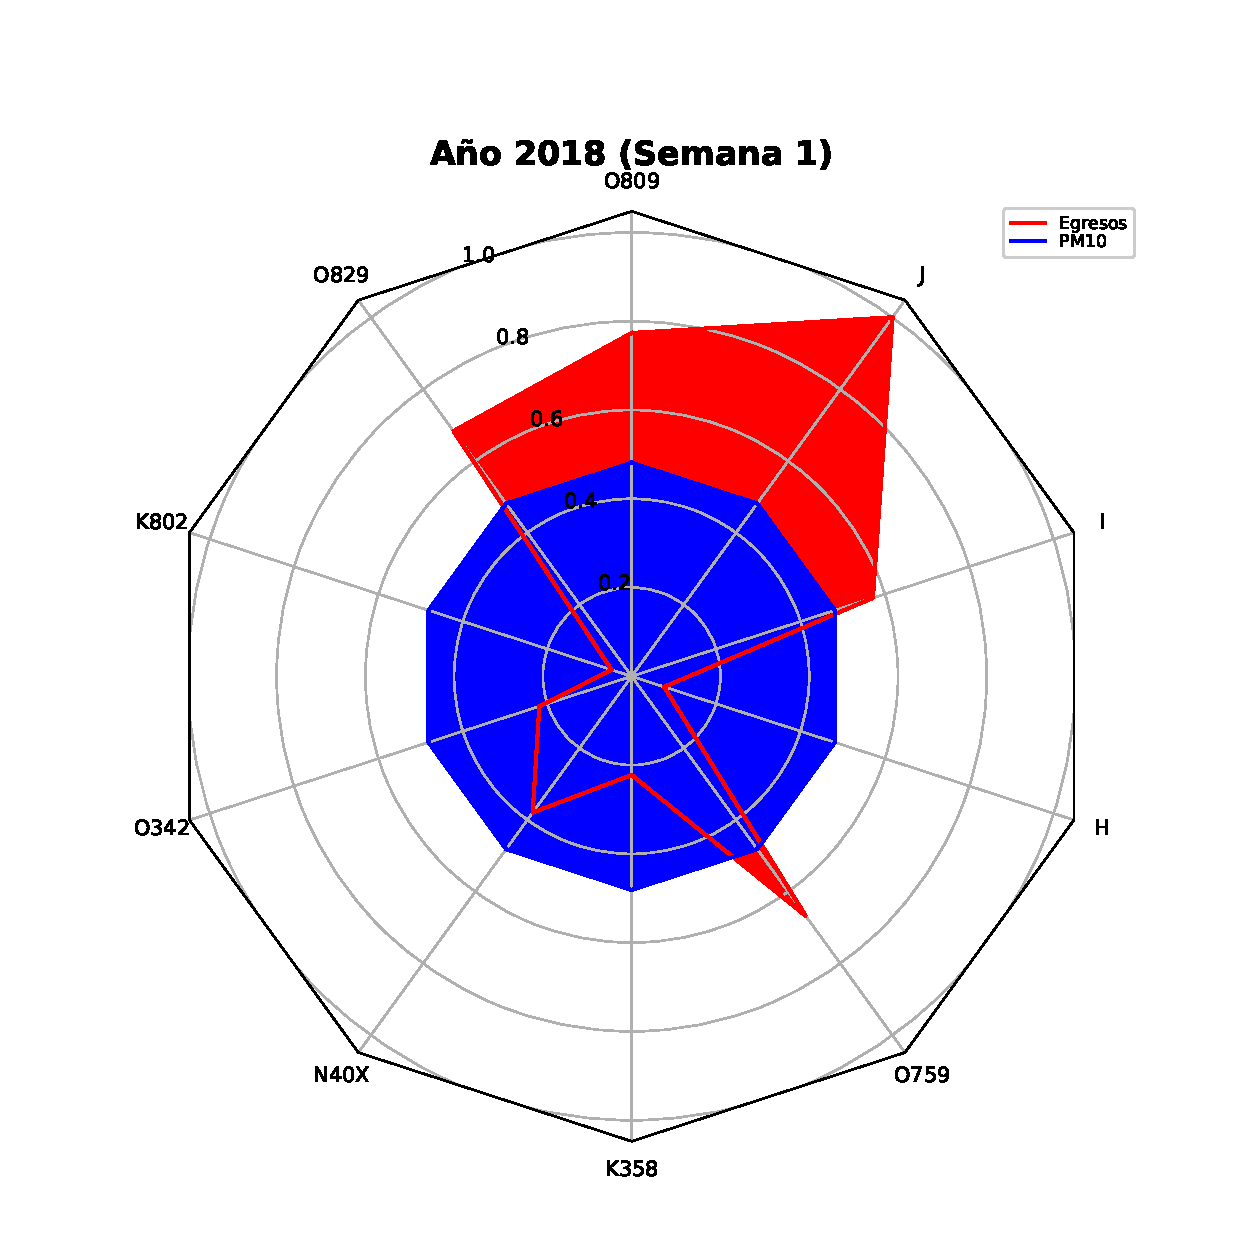
\includegraphics[trim=0 0 0 74,clip,width=0.7\textwidth]{spiderweb_PM10_2018_1.eps}
   \end{center}
    \caption[Ejemplo de gráfico de radar]{Nivel del contaminante PM10 y egresos por CIE en la semana 1 del año 2018.}
    \label{grafico_de_telaraña}
\end{figure}

\clearpage
\section{Experimentos}

En esta sección se presenta el diseño de los experimentos realizados así como los resultados obtenidos de ellos y se tratan los resultados obtenidos partiendo de desarrollar algunos experimentos que permiten determinar si la solución propuesta cumple con el objetivo planteado.

\subsection{Diseño experimental}
En la presente sección se discute el diseño de experimentos, es decir, qué valores constantes fueron utilizados para su realización y por qué se usan dichos valores.

\subsubsection{Datos de entrada}
Los datos de egresos hospitalarios de los años 2017 y 2018 provienen de la base de datos de la Secretaría de Salud del Gobierno de México \cite{f1}. También se tienen registros de los niveles de PM10 y PM2.5 presentes en el área metropolitana de Monterrey, dichos registros son obtenidos por las estaciones de monitoreo pertenecientes al SIMA \cite{f2} mostradas en la figura \ref{estaciones}. Los documentos con los datos son proporcionados por \citet{f3}.

\begin{description}
\item [Selección de datos.] {Los conjuntos de datos por año de egresos hospitalarios contienen información de todos los estados de México, por lo cual se hace una limpieza de datos para solo obtener los registros de Nuevo León ya que de dicha entidad es de la cual se tienen los datos de contaminación.}
\item [Datos de ingresos hospitalarios.] {Se agrupan en semanas epidemiológicas para una mejor manipulación de ellos. Por CIE se obtiene el número de egresos en cada semana del año.}
\item [Datos de los contaminantes.] {Se agrupan en semanas epidemiológicas para una mejor manipulación de ellos. Se obtiene el promedio del nivel del contaminante por cada semana del año.}
\end{description}

\subsubsection{Visualización de datos}
Con los datos ya seleccionados y agrupados se procede a generar las visualizaciones de los datos. Las visualizaciones de los datos se hacen con series de tiempo y gráficos de radar.

\begin{description}
\item [Series de tiempo.] {Se procede a generar series de tiempo de cada año por contaminante y CIE}. Las variables ajustables son:
\begin{itemize}
	\item El nombre del contaminante.
	\item El año del que se quieren obtener las series de tiempo.
	\item Número de series de tiempo a generar por contaminante. Se parte de la CIE con mayor número de egresos.
\end{itemize}

\item [Gráficos de radar.] {Los datos ya seleccionados y agrupados se normalizan teniendo como valor mínimo cero y como valor máximo un número entre uno y cuatro. Posteriormente se generan gráficos de radar de cada año por semana, en las que se muestra el nivel contaminante y la variación de las CIE}. Las variables ajustables son:
\begin{itemize}
    \item Cantidad de CIE a agregar en el gráfico. Se parte de la CIE con mayor número de egresos.
	\item Valor máximo que se utiliza para representar la longitud de los ejes en el gráfico.
	\item Nombre de la figura.
	\item Nombre de cada eje en el gráfico.
	\item Los colores de cada eje en el gráfico. 
	\item Si el gráfico es generado de forma circular o en forma de polígono.
\end{itemize}
\end{description}

\subsubsection{Generación de modelos}
Se procede a generar los modelos. En cada modelo se tienen métricas para evaluar su eficacia y valores que pueden ser ajustados en función de encontrar la combinación que proporcione mejores resultados.

Se tienen algunas variables que pueden ser modificadas para la generación de los modelos de regresión lineal.

\begin{itemize}
	\item Cantidad de CIE a agregar en el modelo. Se parte de la CIE con mayor número de egresos.
	\item Porcentaje de datos utilizados para el entrenamiento del modelo.
	\item Nivel de significancia.
\end{itemize}

También se tienen variables que indican información sobre la eficacia del modelo.

\begin{itemize}
	\item Valor $p$.
	\item $R^2$ (R cuadrado).
	\item Raíz de error cuadrático medio (RMSE).
\end{itemize}


\subsection{Resultados}
Establecidas las especificaciones de los experimentos que se realizan, se reportan los resultados obtenidos. Los experimentos se elaboran por contaminante, desglosando los resultados por año. En la carpeta \url{https://github.com/selenebpradop/relaciones-contaminantes-salud/tree/main/figuras/} se encuentran animaciones en video de los gráficos de radar generados por contaminante y año y todas las imágenes de las series de tiempo obtenidas.

\subsubsection{Experimento A: Datos de niveles de PM10}
Se estudian los niveles del contaminante PM10 de los años 2017 y 2018. 

\begin{description}
\item[Año 2017.]{En la figura \ref{serie_de_tiempo_2017_PM10} se muestra una de las series de tiempo generadas para la CIE con mayor número de egresos registrados en el conjunto de datos del año. Además, en el cuadro \ref{tab:Resultados obtenidos PM10 2017} se presentan los resultados obtenidos de los modelos de regresión lineal y la eficacia obtenida de dichos modelos. El cuadro \ref{tab:RRLM PM10 2017} muestra los resultados del modelo de regresión lineal múltiple.}

\item[Año 2018.]{En la figura \ref{serie_de_tiempo_2018_PM10} se muestra una de las series de tiempo generadas para la CIE con mayor número de egresos registrados en el conjunto de datos del año. Además, en el cuadro \ref{tab:Resultados obtenidos PM10 2018} se presentan los resultados obtenidos de los modelos de regresión lineal y la eficacia obtenida de dichos modelos. El cuadro \ref{tab:RRLM PM10 2018} muestra los resultados del modelo de regresión lineal múltiple.}
\end{description}

\begin{figure}[h!]
\setcounter{figure}{2} % por culpa de sciposter
%\captionsetup{type=figure} % por culpa de sciposter
\begin{center}
   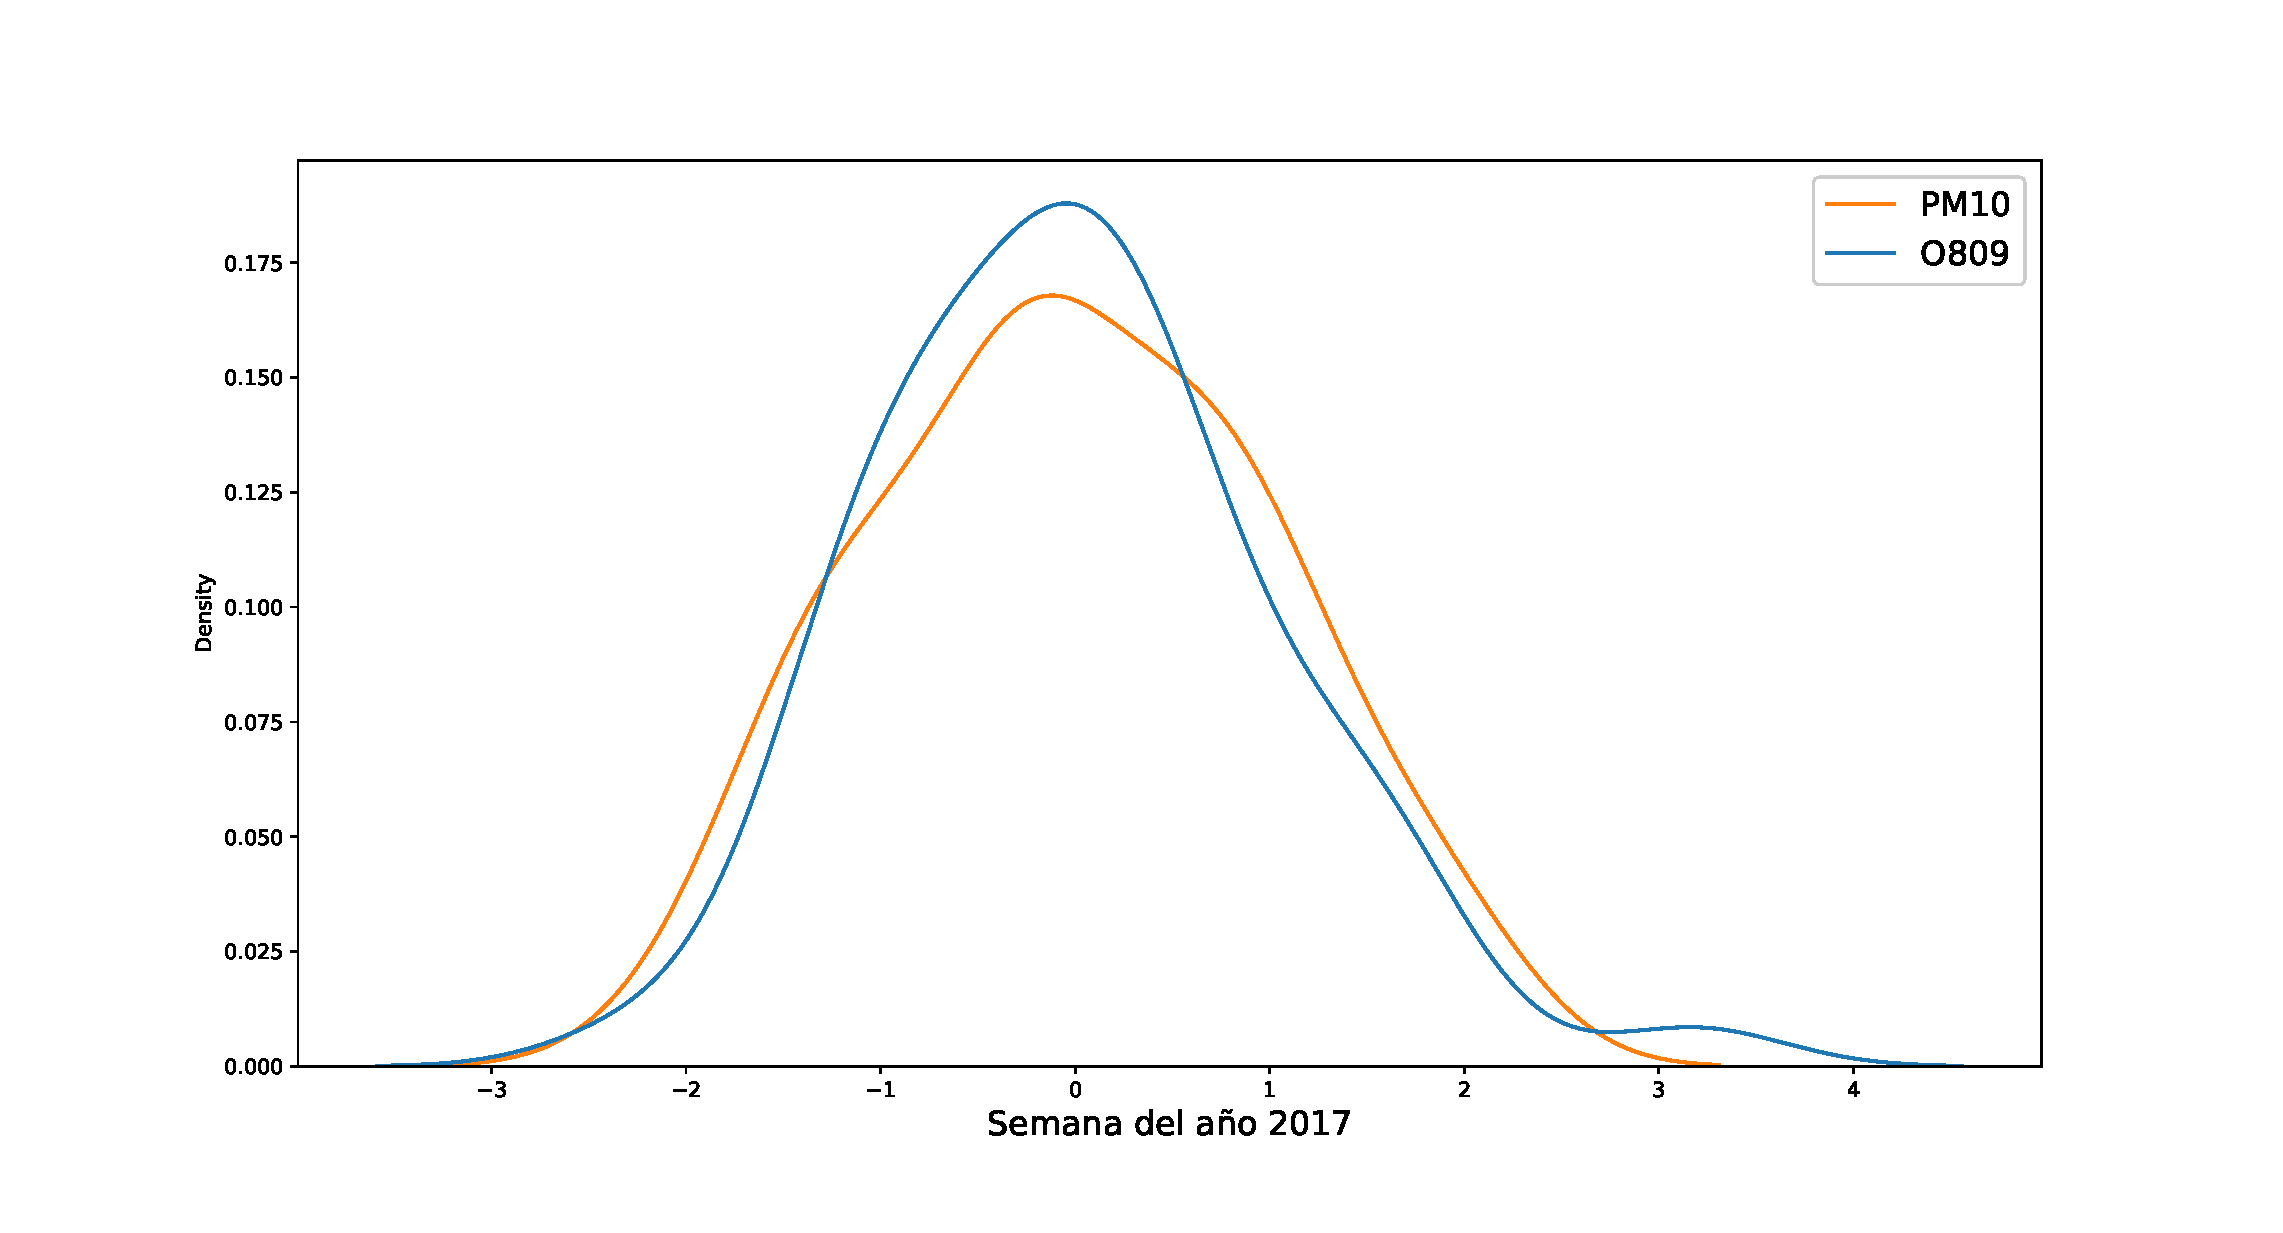
\includegraphics[width=1\textwidth]{PM10_O809_2017.eps}
   \end{center}
    \caption[Series de tiempo 2017 PM10 y O809]{Evolución de los niveles de PM10 y el número de egresos diagnosticados con la CIE O809 en el 2017.}
    \label{serie_de_tiempo_2017_PM10}
\end{figure}

\begin{table}[hbt!]
\centering
\caption{Resultados obtenidos PM10 2017}
\label{tab:Resultados obtenidos PM10 2017}
\vspace{0.5cm}
\begin{threeparttable}
\begin{tabular}{|c|c|c|c|c|}
	\hline
	CIE & $\rho$ & $R^2$ & Valor $p$ & $\epsilon$\\
	\hline
	O809 & -0.275 & 0.061 & 0.121 & 0.239 \\
	\hline
	O829 & 0.100 & 0.091 & 0.055 & 0.287 \\
	\hline
	O759 & -0.085 & 0.116 & 0.029 & 0.294 \\
	\hline
	O069 & -0.247 & 0.070 & 0.094 & 0.222 \\
	\hline
	K802 & 0.044 & 0.005 & 0.658 & 0.282 \\
	\hline
\end{tabular}
\begin{tablenotes}
\footnotesize
\item{$\rho$ = Coeficiente de correlación de Pearson}
\item{$\epsilon$ = RMSE para medir el error}
\end{tablenotes}
\end{threeparttable}
\end{table}

\begin{table}[hbt!]
\caption{Resultados regresión lineal múltiple PM10 2017}
\label{tab:RRLM PM10 2017}
\begin{center}
\begin{tabular}{lclc}
\toprule
\textbf{Variable Dep.:}    &        $y$         & \textbf{  R$^2$:         } &     0.313   \\
\textbf{Modelo:}            &       OLS        & \textbf{Método:}           &  Mínimos cuadrados  \\
\textbf{Error:}            & 0.226  \\
\bottomrule
\end{tabular}
\begin{tabular}{lcccccc}
               & \textbf{coef} & \textbf{std err} & \textbf{$t$} & \textbf{P$> |$t$|$} & \textbf{[0.025} & \textbf{0.975]}  \\
\midrule
\textbf{const} &       0.5859  &        0.146     &     4.002  &         0.000        &        0.289    &        0.883     \\
\textbf{O809}  &      -0.3019  &        0.122     &    -2.472  &         0.018        &       -0.550    &       -0.054     \\
\textbf{O829}  &       0.2685  &        0.123     &     2.185  &         0.036        &        0.019    &        0.518     \\
\textbf{O759}  &      -0.2229  &        0.182     &    -1.222  &         0.230        &       -0.593    &        0.147     \\
\textbf{O069}  &      -0.1441  &        0.120     &    -1.200  &         0.238        &       -0.388    &        0.100     \\
\textbf{K802}  &      -0.0456  &        0.133     &    -0.344  &         0.733        &       -0.315    &        0.224     \\
\bottomrule
\end{tabular}
\end{center}
\end{table}

\begin{figure}[h!]
\setcounter{figure}{3} % por culpa de sciposter
%\captionsetup{type=figure} % por culpa de sciposter
\begin{center}
   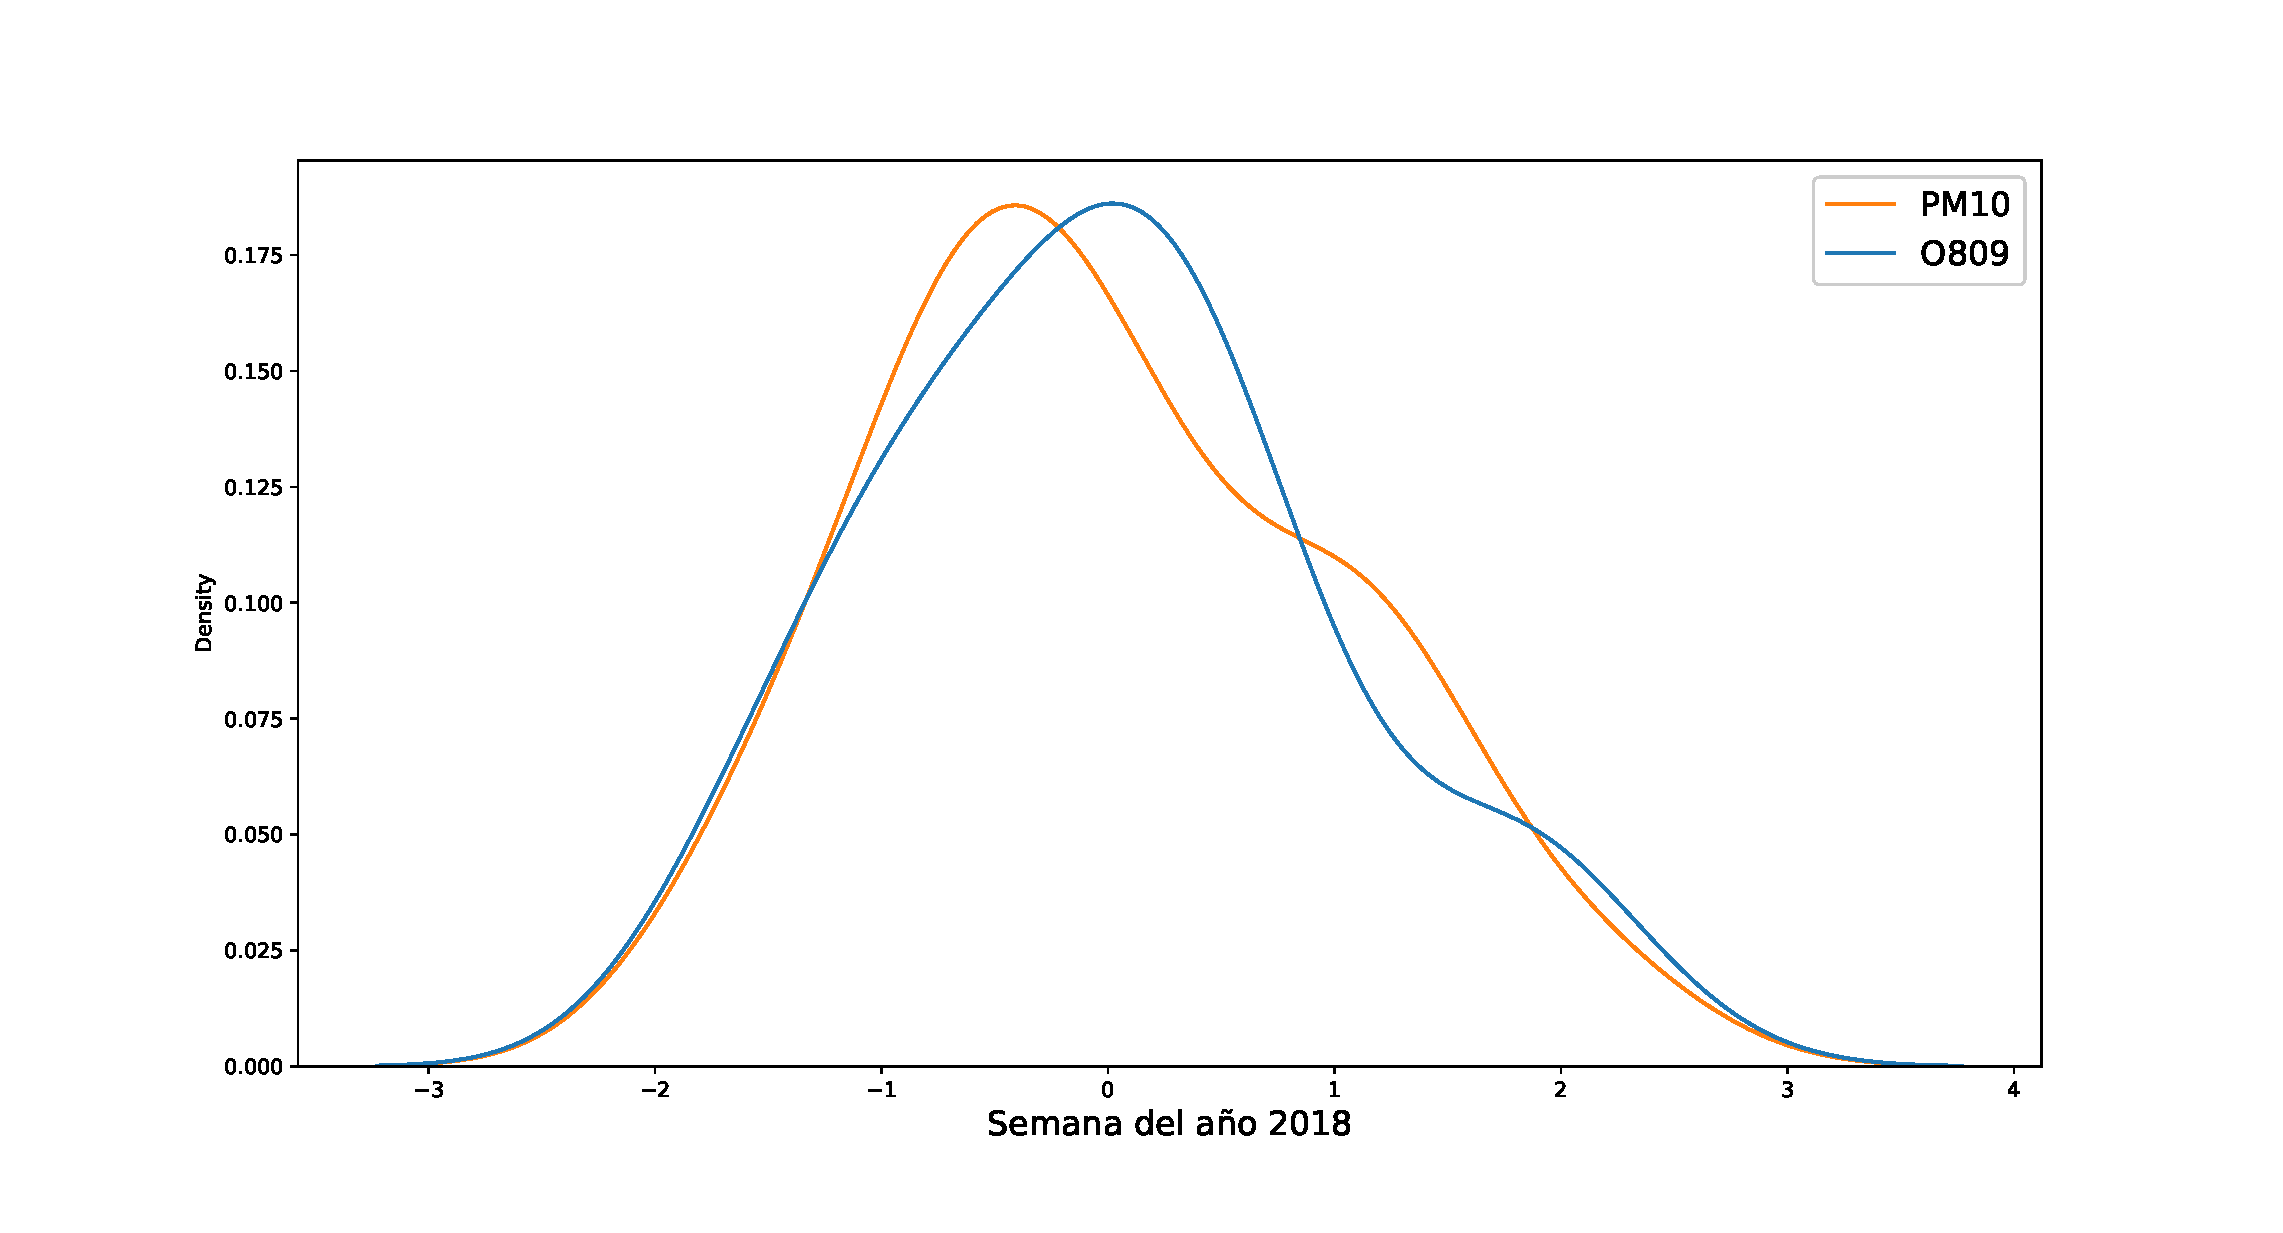
\includegraphics[width=1\textwidth]{PM10_O809_2018.eps}
   \end{center}
    \caption[Series de tiempo 2018 PM10 y O809]{Evolución de los niveles de PM10 y el número de egresos diagnosticados con la CIE O809 en el 2018.}
    \label{serie_de_tiempo_2018_PM10}
\end{figure}

\begin{table}[hbt!]
\centering
\caption{Resultados obtenidos PM10 2018}
\label{tab:Resultados obtenidos PM10 2018}
\vspace{0.5cm}
\begin{threeparttable}
\begin{tabular}{|c|c|c|c|c|}
	\hline
	CIE & $\rho$ & $R^2$ & Valor $p$ & $\epsilon$\\
	\hline
	O809 & -0.271 & 0.015 & 0.440 & 0.275 \\
	\hline
	O829 & 0.282 & 0.069 & 0.098 & 0.249 \\
	\hline
	K802 & 0.277 & 0.084 & 0.066 & 0.152 \\
	\hline
	O342 & -0.401 & 0.100 & 0.044 & 0.248 \\
	\hline
	N40X & -0.009 & 0.000 & 0.964 & 0.243 \\
	\hline
\end{tabular}
\begin{tablenotes}
\footnotesize
\item{$\rho$ = Coeficiente de correlación de Pearson}
\item{$\epsilon$ = RMSE para medir el error}
\end{tablenotes}
\end{threeparttable}
\end{table}

\begin{table}[hbt!]
\caption{Resultados regresión lineal múltiple PM10 2018}
\label{tab:RRLM PM10 2018}
\begin{center}
\begin{tabular}{lclc}
\toprule
\textbf{Variable Dep.:}    &        $y$         & \textbf{  R$^2$:         } &     0.182   \\
\textbf{Modelo:}            &       OLS        & \textbf{Método:}           &  Mínimos cuadrados  \\
\textbf{Error:}            & 0.159  \\
\bottomrule
\end{tabular}
\begin{tabular}{lcccccc}
               & \textbf{coef} & \textbf{std err} & \textbf{$t$} & \textbf{P$> |$t$|$} & \textbf{[0.025} & \textbf{0.975]}  \\
\midrule
\textbf{const} &       0.3885  &        0.210     &     1.849  &         0.073        &       -0.038    &        0.815     \\
\textbf{O809}  &      -0.0114  &        0.188     &    -0.061  &         0.952        &       -0.392    &        0.370     \\
\textbf{O829}  &       0.0854  &        0.214     &     0.400  &         0.692        &       -0.349    &        0.520     \\
\textbf{K802}  &       0.3088  &        0.167     &     1.852  &         0.072        &       -0.030    &        0.647     \\
\textbf{O342}  &      -0.1708  &        0.208     &    -0.820  &         0.418        &       -0.593    &        0.252     \\
\textbf{N40X}  &      -0.1239  &        0.167     &    -0.740  &         0.464        &       -0.464    &        0.216     \\
\bottomrule
\end{tabular}
\end{center}
\end{table}

\clearpage
\subsubsection{Experimento B: Niveles de PM2.5}
Se estudian los niveles del contaminante PM2.5 de los años 2017 y 2018.

\begin{description}
\item[Año 2017.]{En la figura \ref{serie_de_tiempo_2017_PM25} se muestra una de las series de tiempo generadas para la CIE con mayor número de egresos registrados en el conjunto de datos del año. Además, en el cuadro \ref{tab:Resultados obtenidos PM2.5 2017} se presentan los resultados obtenidos de los modelos de regresión lineal y la eficacia obtenida de dichos modelos. El cuadro \ref{tab:RRLM PM2.5 2017} muestra los resultados del modelo de regresión lineal múltiple.}

\item[Año 2018.]{En la figura \ref{serie_de_tiempo_2018_PM25} se muestra una de las series de tiempo generadas para la CIE con mayor número de egresos registrados en el conjunto de datos del año. Además, en el cuadro \ref{tab:Resultados obtenidos PM2.5 2018} se presentan los resultados obtenidos de los modelos de regresión lineal y la eficacia obtenida de dichos modelos. El cuadro \ref{tab:RRLM PM2.5 2018} muestra los resultados del modelo de regresión lineal múltiple.}
\end{description}

\begin{figure}[h!]
\setcounter{figure}{4} % por culpa de sciposter
%\captionsetup{type=figure} % por culpa de sciposter
\begin{center}
   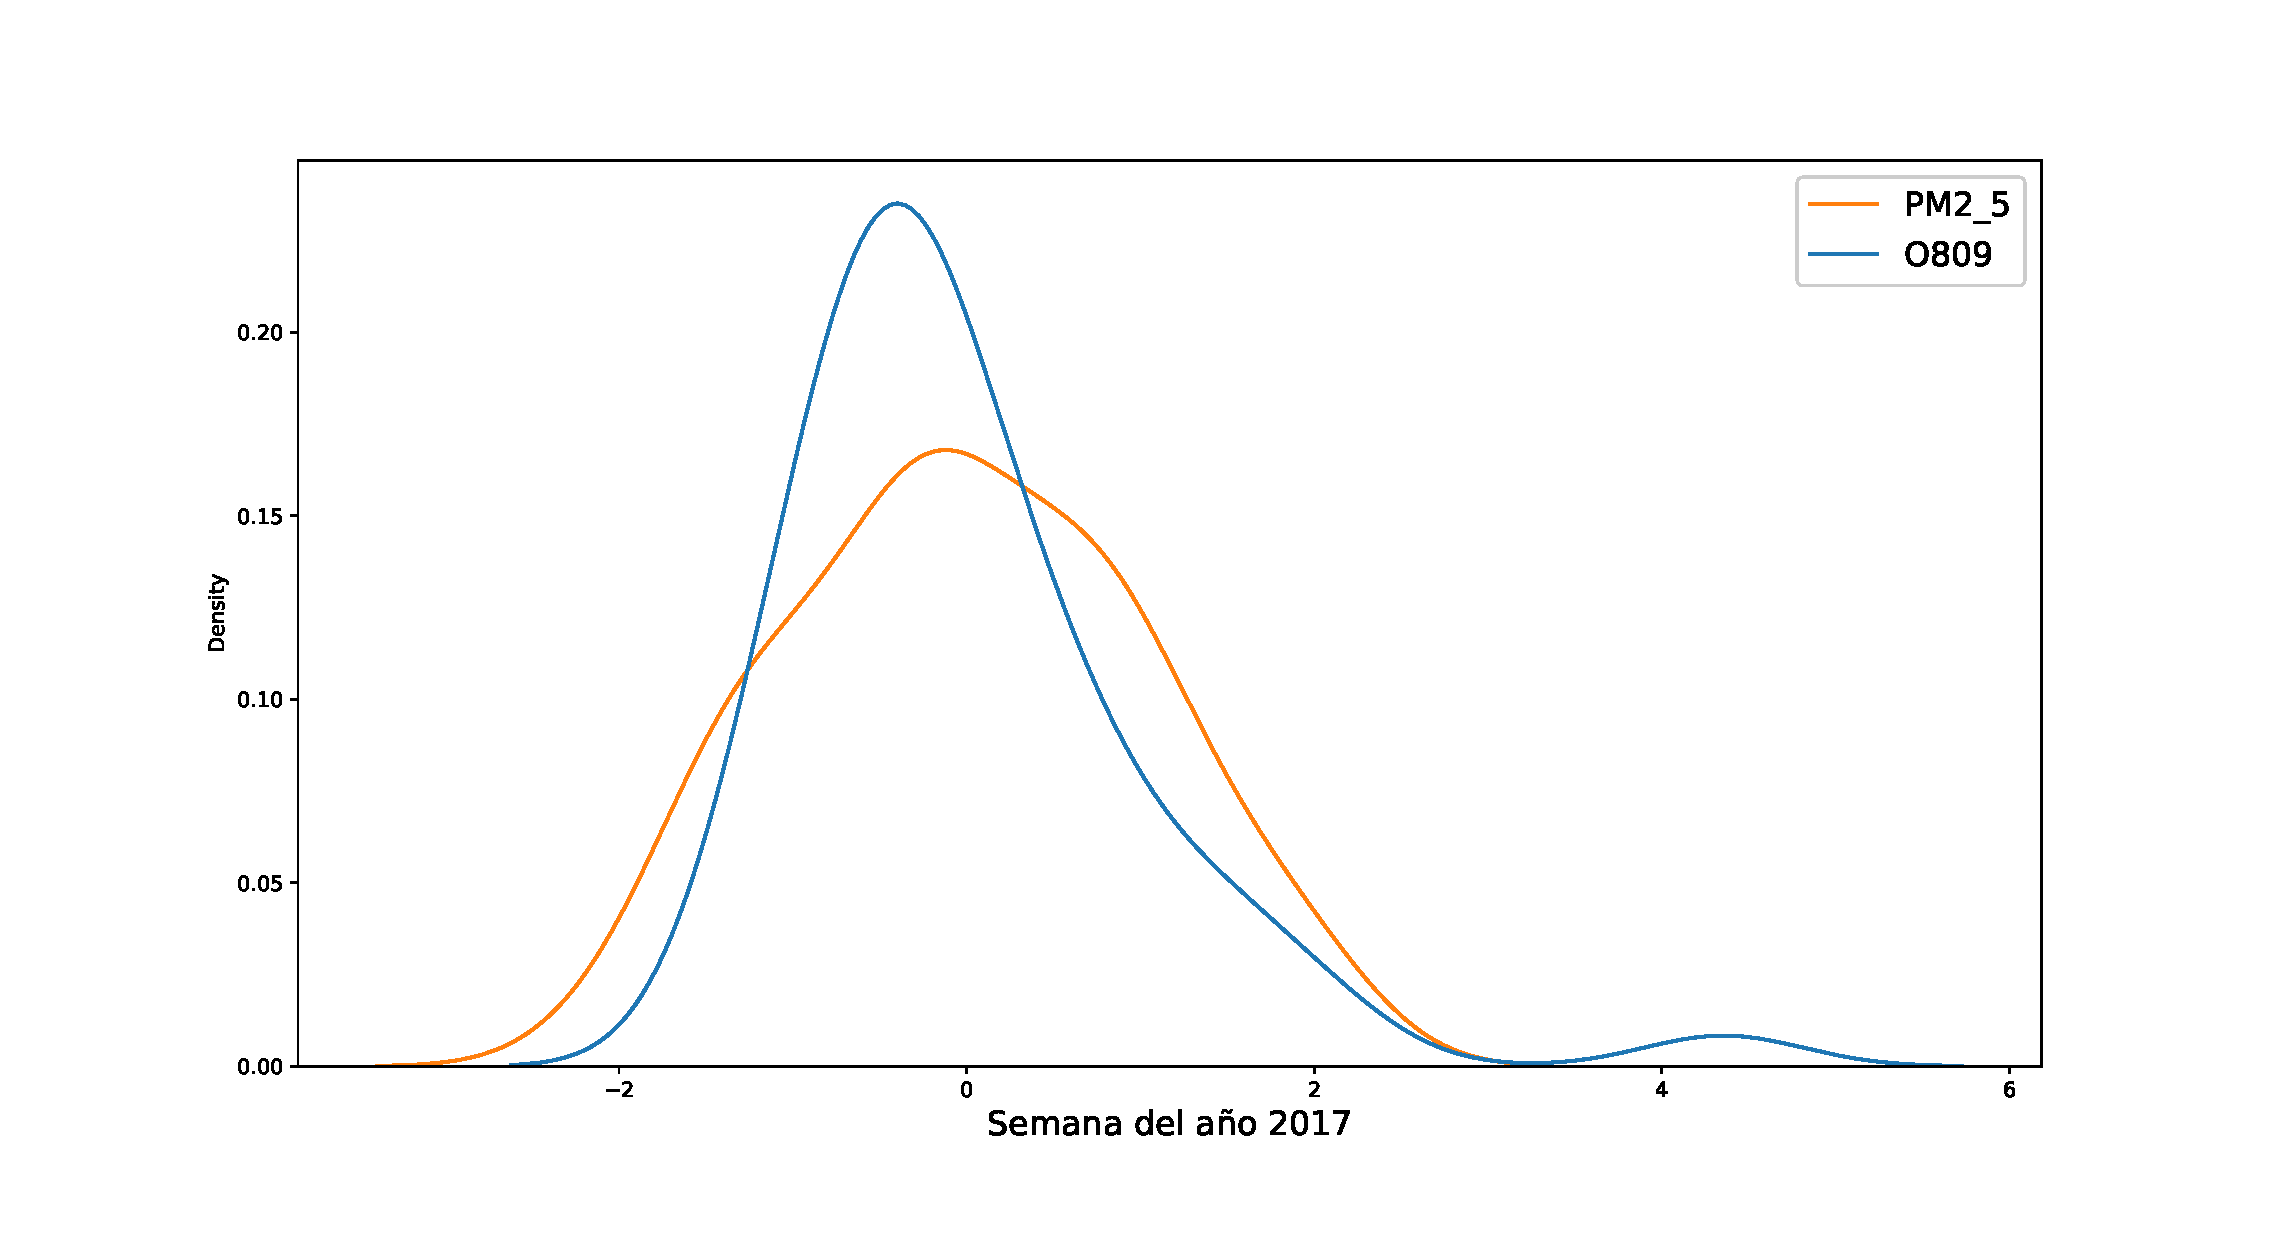
\includegraphics[width=1\textwidth]{PM2_5_O809_2017.eps}
   \end{center}
    \caption[Series de tiempo 2017 PM2.5 y O809]{Evolución de los niveles de PM2.5 y el número de egresos diagnosticados con la CIE O809 en el 2017.}
    \label{serie_de_tiempo_2017_PM25}
\end{figure}

\begin{table}[hbt!]
\centering
\caption{Resultados obtenidos PM2.5 2017}
\label{tab:Resultados obtenidos PM2.5 2017}
\vspace{0.5cm}
\begin{threeparttable}
\begin{tabular}{|c|c|c|c|c|}
	\hline
	CIE & $\rho$ & $R^2$ & Valor $p$ & $\epsilon$\\
	\hline
	O809 & -0.093 & 0.011 & 0.511 & 0.256 \\
	\hline
	O829 & 0.014 & 0.021 & 0.371 & 0.253 \\
	\hline
	O759 & -0.172 & 0.113 & 0.032 & 0.278 \\
	\hline
	O069 & -0.350 & 0.112 & 0.033 & 0.208 \\
	\hline
	K802 & 0.006 & 0.005 & 0.667 & 0.285 \\
	\hline
\end{tabular}
\begin{tablenotes}
\footnotesize
\item{$\rho$ = Coeficiente de correlación de Pearson}
\item{$\epsilon$ = RMSE para medir el error}
\end{tablenotes}
\end{threeparttable}
\end{table}

\begin{table}[hbt!]
\caption{Resultados regresión lineal múltiple PM2.5 2017}
\label{tab:RRLM PM2.5 2017}
\begin{center}
\begin{tabular}{lclc}
\toprule
\textbf{Variable Dep.:}    &        $y$         & \textbf{  R$^2$:         } &     0.210   \\
\textbf{Modelo:}            &       OLS        & \textbf{Método:}           &  Mínimos cuadrados   \\
\textbf{Error:}            & 0.175  \\
\bottomrule
\end{tabular}
\begin{tabular}{lcccccc}
               & \textbf{coef} & \textbf{std err} & \textbf{$t$} & \textbf{P$> |$t$|$} & \textbf{[0.025} & \textbf{0.975]}  \\
\midrule
\textbf{const} &       0.5345  &        0.158     &     3.373  &         0.002        &        0.213    &        0.856     \\
\textbf{O809}  &      -0.1754  &        0.132     &    -1.327  &         0.193        &       -0.444    &        0.093     \\
\textbf{O829}  &       0.0701  &        0.133     &     0.527  &         0.602        &       -0.200    &        0.340     \\
\textbf{O759}  &      -0.2585  &        0.197     &    -1.309  &         0.199        &       -0.659    &        0.142     \\
\textbf{O069}  &      -0.2148  &        0.130     &    -1.652  &         0.108        &       -0.479    &        0.049     \\
\textbf{K802}  &      -0.1164  &        0.144     &    -0.811  &         0.423        &       -0.408    &        0.175     \\
\bottomrule
\end{tabular}
\end{center}
\end{table}

\begin{figure}[h!]
\setcounter{figure}{5} % por culpa de sciposter
%\captionsetup{type=figure} % por culpa de sciposter
\begin{center}
   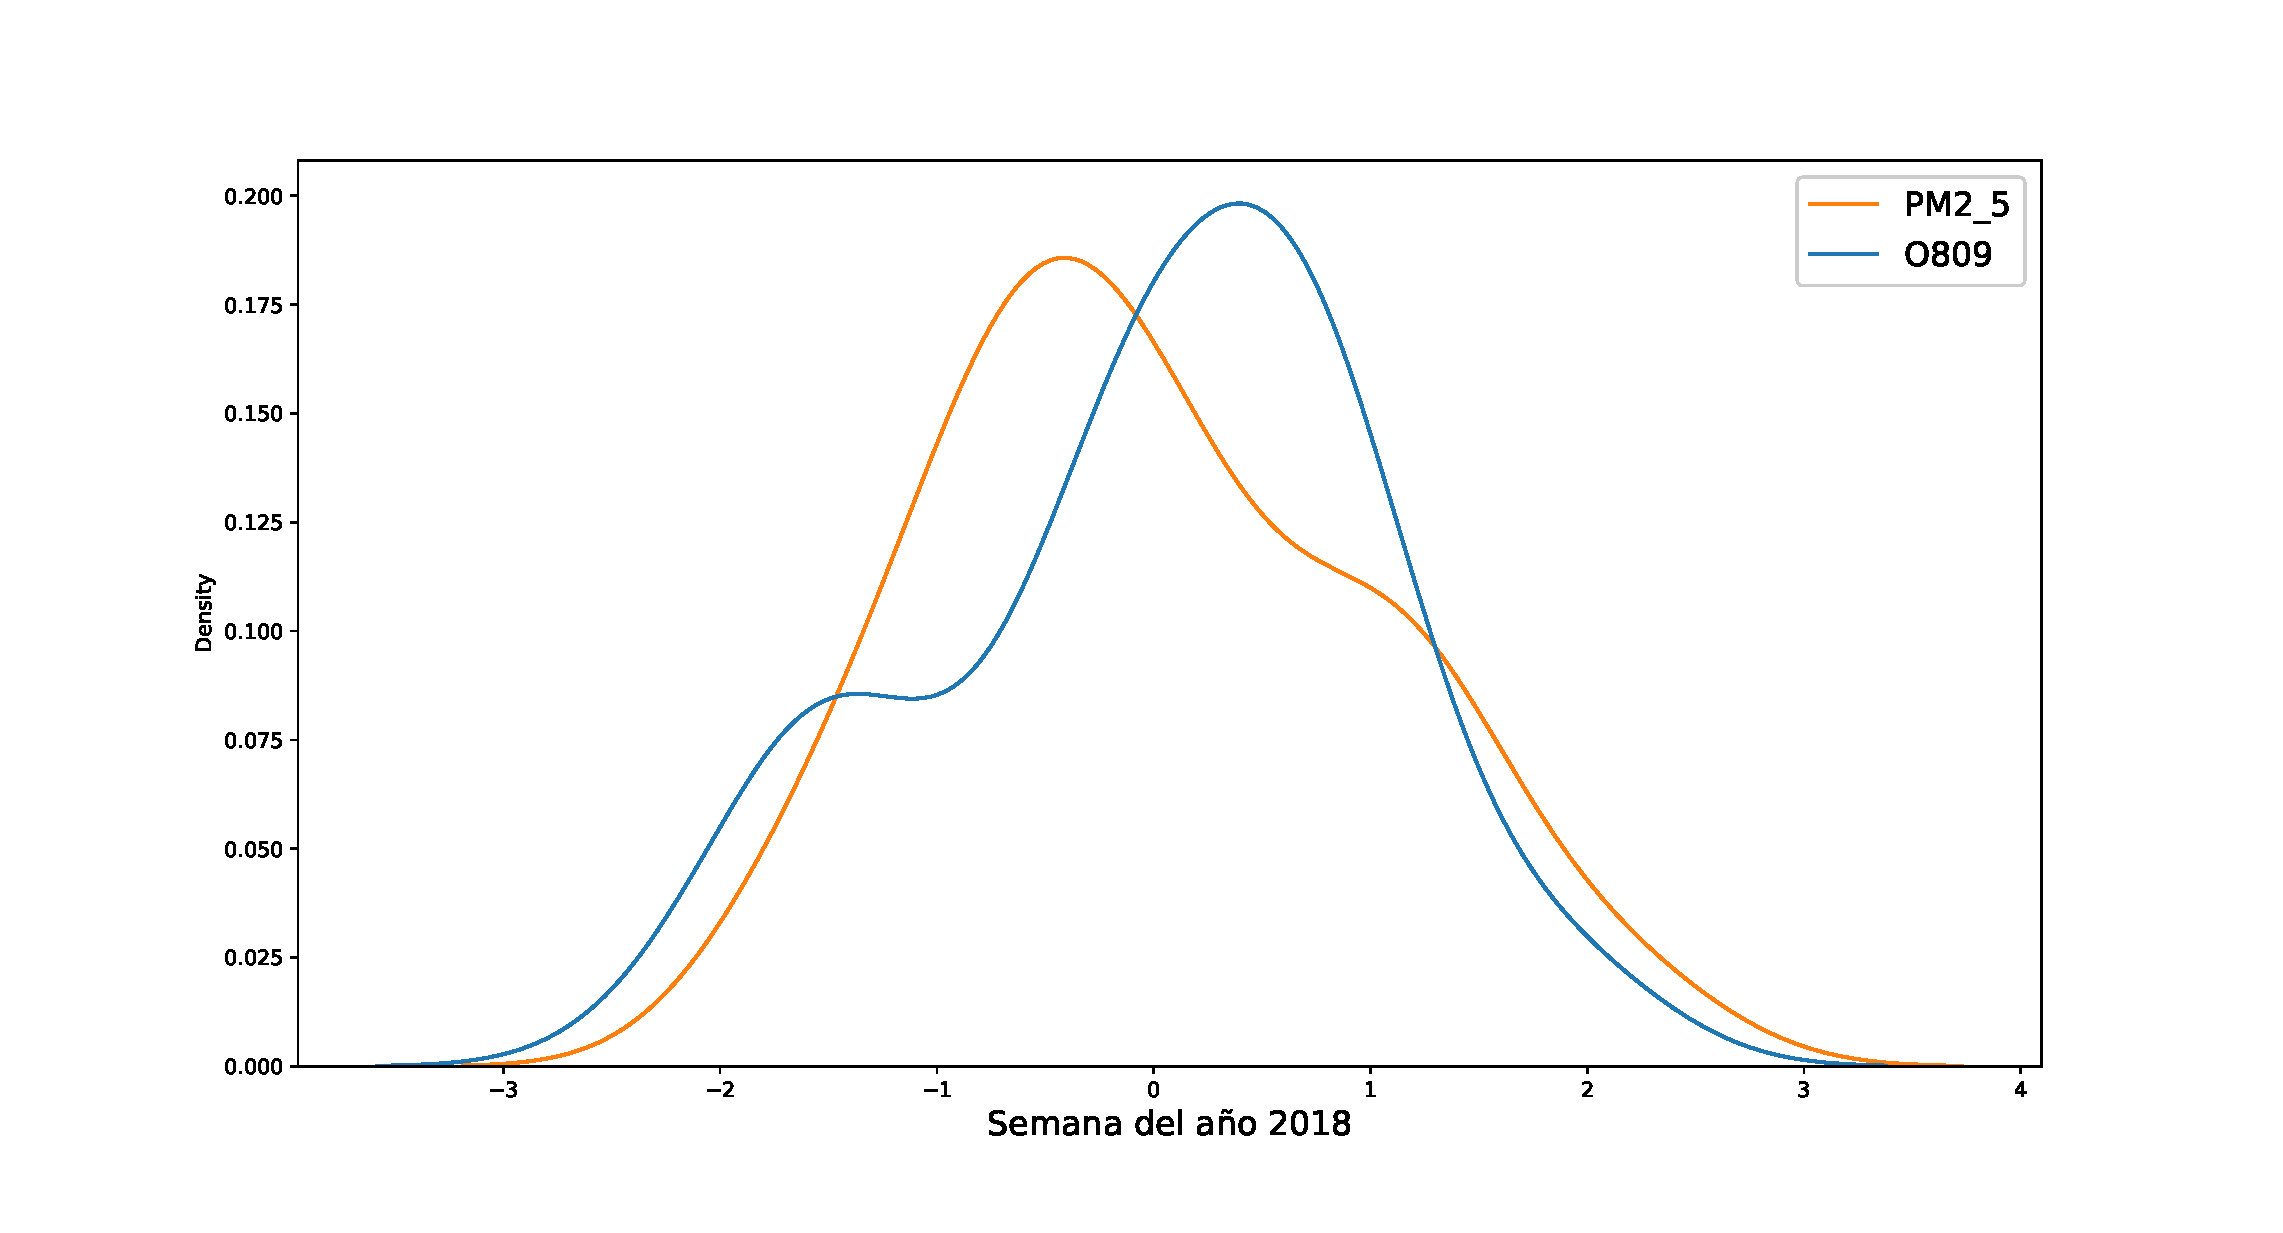
\includegraphics[width=1\textwidth]{PM2_5_O809_2018.eps}
   \end{center}
    \caption[Series de tiempo 2018 PM2.5 y O809]{Evolución de los niveles de PM2.5 y el número de egresos diagnosticados con la CIE O809 en el 2018.}
    \label{serie_de_tiempo_2018_PM25}
\end{figure}

\begin{table}[hbt!]
\centering
\caption{Resultados obtenidos PM2.5 2018}
\label{tab:Resultados obtenidos PM2.5 2018}
\vspace{0.5cm}
\begin{threeparttable}
\begin{tabular}{|c|c|c|c|c|}
	\hline
	CIE & $\rho$ & $R^2$ & Valor $p$ & $\epsilon$\\
	\hline
	O809 & -0.354 & 0.057 & 0.133 & 0.259 \\
	\hline
	O829 & 0.225 & 0.046 & 0.177 & 0.256 \\
	\hline
	K802 & 0.273 & 0.089 & 0.058 & 0.159 \\
	\hline
	O342 & -0.443 & 0.149 & 0.013 & 0.245 \\
	\hline
	N40X & -0.074 & 0.001 & 0.842 & 0.241 \\
	\hline
\end{tabular}
\begin{tablenotes}
\footnotesize
\item{$\rho$ = Coeficiente de correlación de Pearson}
\item{$\epsilon$ = RMSE para medir el error}
\end{tablenotes}
\end{threeparttable}
\end{table}

\begin{table}[hbt!]
\caption{Resultados regresión lineal múltiple PM2.5 2018}
\label{tab:RRLM PM2.5 2018}
\begin{center}
\begin{tabular}{lclc}
\toprule
\textbf{Variable Dep.:}    &        $y$         & \textbf{  R$^2$:         } &     0.259   \\
\textbf{Modelo:}            &       OLS        & \textbf{Método:}           &  Mínimos cuadrados   \\
\textbf{Error:}            & 0.174  \\
\bottomrule
\end{tabular}
\begin{tabular}{lcccccc}
               & \textbf{coef} & \textbf{std err} & \textbf{$t$} & \textbf{P$> |$t$|$} & \textbf{[0.025} & \textbf{0.975]}  \\
\midrule
\textbf{const} &       0.7042  &        0.193     &     3.652  &         0.001        &        0.313    &        1.096     \\
\textbf{O809}  &      -0.0863  &        0.172     &    -0.501  &         0.620        &       -0.436    &        0.264     \\
\textbf{O829}  &      -0.1084  &        0.196     &    -0.553  &         0.584        &       -0.507    &        0.290     \\
\textbf{K802}  &       0.3006  &        0.153     &     1.964  &         0.058        &       -0.010    &        0.611     \\
\textbf{O342}  &      -0.3311  &        0.191     &    -1.733  &         0.092        &       -0.719    &        0.057     \\
\textbf{N40X}  &      -0.2053  &        0.154     &    -1.336  &         0.190        &       -0.517    &        0.107     \\
\bottomrule
\end{tabular}
\end{center}
\end{table}

\clearpage
\subsection{Discusión}

Como se puede observar, en todos los experimentos se obtiene una correlación entre -1 y 1 y diferente a 0, por lo tanto se pueden generar los modelos de regresión lineal.

En el Experimento A el error RMSE en los modelos de regresión lineal varía entre 0.152 y 0.294, lo cual indica que no todos los resultados alcanzan una fiabilidad mayor al 80\%, excepto en la CIE K802 en el año 2018 en la cual se encuentra el porcentaje de error más bajo. 
El valor de $R^2$ más alto en el año 2017 se encuentra en la CIE O759 con un valor $p$ de 0.029, sin embargo, en el modelo de regresión lineal múltiple se encuentra el valor de $R^2$ más alto para el contaminante PM10 en el año 2017. En el año 2018 el valor de $R^2$ más alto se encuentra en la CIE O342 con un valor $p$ de 0.044, sin embargo, en el modelo de regresión lineal múltiple se encuentra el valor de $R^2$ más alto para el contaminante PM10 en el año 2018.

En el Experimento B el error RMSE en los modelos de regresión lineal varía entre 0.159 y 0.278, lo cual indica que no todos los resultados alcanzan una fiabilidad mayor al 80\%, excepto en la CIE K802 en el año 2018 en la cual se encuentra el porcentaje de error más bajo.
El valor de $R^2$ más alto en el año 2017 se encuentra en la CIE O759 con un valor $p$ de 0.032, sin embargo, en el modelo de regresión lineal múltiple se encuentra el valor de $R^2$ más alto para el contaminante PM2.5 en el año 2017. En el año 2018 el valor de $R^2$ más alto se encuentra en la CIE O342 con un valor $p$ de 0.013, sin embargo, en el modelo de regresión lineal múltiple se encuentra el valor de $R^2$ más alto para el contaminante PM2.5 en el año 2018.


\section{Conclusiones}

En el presente proyecto se generaron visualizaciones para el estudio de las relaciones entre determinados contaminantes y determinadas CIE. Además, se generaron modelos de regresión lineal y modelos de regresión lineal múltiple con diferentes contaminantes y diferentes CIE para poder realizar una comparación entre los modelos generados.

En los experimentos se encontró un coeficiente de correlación de Pearson diferente a 0 entre -1 y 1, por lo tanto se pudieron generar los modelos de regresión lineal. Se encontró que al estudiar las CIE de manera agrupada en un modelo de regresión múltiple se obtiene una mejor explicación de la varianza de los niveles de los contaminantes PM10 y PM2.5 frente al modelo de regresión lineal simple. Cinco de los veinticuatro valores de error RMSE reportados son menores a 0.20, lo cual indica que la mayoría de los valores predichos por los modelos se alejaron más de 0.20 unidades de los valores reales, por lo tanto dichos valores de error son mayores a los deseados.

Primeramente se encontró que la CIE que reporta mayor número de egresos en Nuevo León, México en los años 2017 y 2018 es la CIE O809. En las series de tiempo se observa que la cantidad de egresos de la mayoría de las CIE estudiadas presentar una línea de evolución similar al contaminante PM10.

Además, se encontró una correlación lineal entre los contaminantes estudiados y las CIE estudiadas, por lo cual el presente proyecto motiva a seguir realizando labores en torno a la investigación de la dependencia lineal que se presenta entre los contaminantes y las CIE.

Finalmente, se observó que para el estudio de las relaciones entre los contaminantes y las CIE se obtuvieron mejores resultados con los modelos de regresión lineal frente a los modelos de regresión lineal simple, lo cual indica que se puede obtener información relevante si se emplean modelos de regresión lineal múltiple para realizar investigaciones que estudien las relaciones entre los niveles de determinados contaminantes y el número de egresos por determinadas CIE.

El presente trabajo brinda algunos aspectos a considerar para realizar un trabajo a futuro, los cuales son: la recolección de más datos de los niveles de contaminantes y de egresos para el estudio de años más recientes, realizar un estudio de las relaciones de los niveles de determinados contaminantes y la cantidad de egresos por CIE empleando modelos de regresión lineal múltiple, la creación de un mapa interactivo donde se pueda observar por región los niveles de los contaminantes y la cantidad de egresos, y la generación de una página web que funcione en conjunto con el desarrollo elaborado para que al ingresar el archivo con los datos se generen las visualizaciones y modelos.

Las oportunidades de mejora detectada para el presente proyecto son: comparar los resultados obtenidos de los modelos regresión lineal múltiple con el mismo modelo pero incrementando el número de variables independientes (CIE), elaborar modelos de regresión no lineal para comparar sus resultados con los resultados de los modelos generados, y utilizar un conjunto de datos más consistente ya que eso favorece a que se tengan resultados más fiables y precisos.


%% The Appendices part is started with the command \appendix;
%% appendix sections are then done as normal sections
%% \appendix

%% \section{}
%% \label{}

%% References
%%
%% Following citation commands can be used in the body text:
%% Usage of \cite is as follows:
%%   \cite{key}         ==>>  [#]
%%   \cite[chap. 2]{key} ==>> [#, chap. 2]
%%

%% References with BibTeX database:

\bibliographystyle{mighelnat}
\bibliography{MiBiblio}

%% Authors are advised to use a BibTeX database file for their reference list.
%% The provided style file elsarticle-num.bst formats references in the required Procedia style

%% For references without a BibTeX database:

% \begin{thebibliography}{00}

%% \bibitem must have the following form:
%%   \bibitem{key}...
%%

% \bibitem{}

% \end{thebibliography}

\end{document}

%%
%% End of file `ecrc-template.tex'. 